

\chapter{Ansatz Methods and Weak Solutions}

Up to this point in the course we have mostly represented the solutions of ODEs (either IVP or BVP) on some interval $[a, b] \subseteq \R$ 
using {\it mesh functions}, effectively storing the numerical solution 
$\ub = (u_0, \dots, u_N) \approx
(u(t_0), \dots, u(t_N))$ for a grid $t_0, \dots, t_N$ in the interval on which 
the problem was defined. Stepping back for a second we realize that $\ub$ is a vector in 
$\R^{N+1}$ or $\C^{N+1}$ while the true solutions to our problem are functions $u: [a, b] \to \R$ (or $\C$). Thus we have an inconsistency between the kind of object our algorithm produces (i.e., $\ub$) and what we are trying to approximate (i.e., $u$). 
Put another way, what if we want to extract an approximation to $u(t)$ for some $t \in (t_n, t_{n+1})$? Well, a natural approach would be to construct an approximation 
to $u(t)$ given the numerical estimates $u_n$ and $u_{n+1}$. A simple approach would be to 
use  a piecewise linear interpolant, see \Cref{fig:piecewise-linear-interpolant-demo},
\begin{equation*}
    \hat{u}(t) = \frac{u_{n+1} - u_n}{t_{n+1} - t_n} (t- t_n) + u_n \quad \text{if} \quad t \in [t_n, t_{n+1}).  
\end{equation*}
Now $\hat{u}$ is a proper function on the interval $[a,b]$ and, mathematically, it is the 
object that we were after all along. 

\begin{figure}[htp]
    \centering
    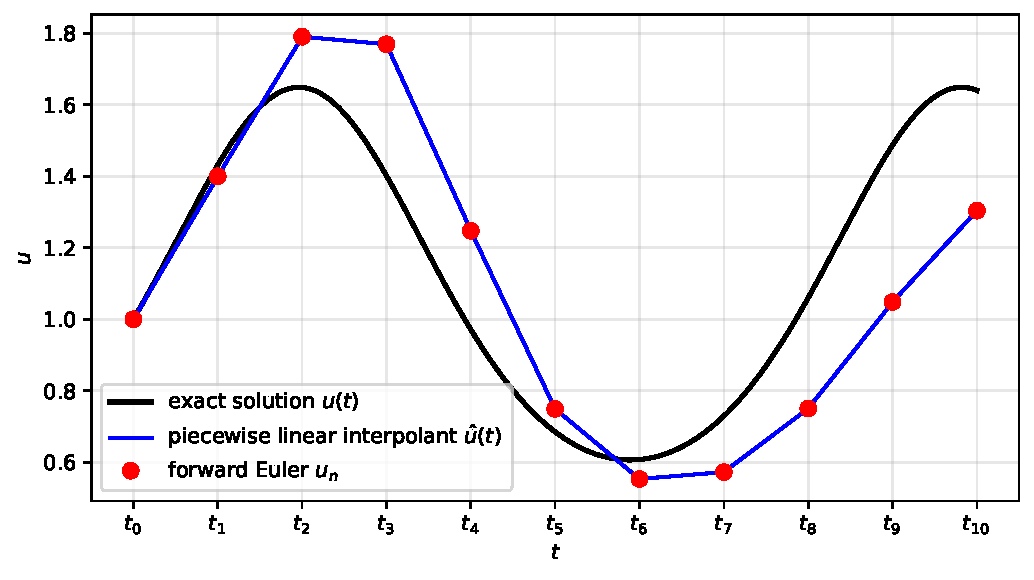
\includegraphics[width=0.65\textwidth]{./Lectures/Lec19/piecewise_linear_interpolant_demo.pdf}
    \caption{Comparison of the true solution of an example IVP (black curve) with the forward Euler output $\ub$ (red dots) and the subsequent piecewise linear interpolant $\hat{u}$ (blue).}
    \label{fig:piecewise-linear-interpolant-demo}
\end{figure}

Let us define the hat functions $\phi_n$, see \Cref{fig:hat-functions},
\begin{equation*}
\begin{aligned}
    \phi_0(t) &= \left\{
        \begin{aligned}
            & \frac{t_1 - t}{t_1 - t_0} && t \in[t_0, t_1] \\ 
            & 0 && \text{otherwise}, 
        \end{aligned}
    \right. \\
    \phi_{n}(t)& = \left\{
         \begin{aligned}
            & \frac{t - t_{n-1}}{t_n - t_{n-1}} && t \in[t_{n-1}, t_n] \\
            & \frac{t_{n+1} - t}{t_{n+1} - t_n} && t \in[t_n, t_{n+1}] \\ 
            & 0 && \text{otherwise}, 
        \end{aligned}
    \right. \\
    \phi_N(t) &= \left\{
        \begin{aligned}
            & \frac{t - t_{N-1}}{t_N - t_{N-1}} && t \in[t_{N-1}, t_N] \\ 
            & 0 && \text{otherwise}, 
        \end{aligned}
    \right.
\end{aligned}
\end{equation*}
\begin{figure}[htp]
    \centering
    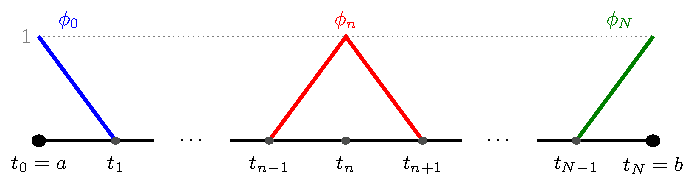
\includegraphics{./Lectures/Lec19/hat_functions.pdf}
    \caption{A plot of the hat functions $\phi_n$. Notice that these functions 
    are equal to $1$ at the mesh point $t_n$ and zero at all other mesh points.}
    \label{fig:hat-functions}
\end{figure}
Then we can show, with a little bit of algebra left for your homework, that 
\begin{equation*}
    \hat{u}(t) = \sum_{n=0}^N u_n \phi_n(t).
\end{equation*}
The above observation is the key idea underlying ansatz methods for solving BVPs and later 
for PDEs. Linear ansatz methods proceed by assuming that 
the numerical solution to the BVP can be written as 
\begin{equation}\label{eq:l18:u-linear-expansion}
    \hat{u}(t) = \sum_{n=0}^N c_n \varphi_n(t),
\end{equation}
where $\varphi_n: [a, b] \to \R$ (or $\C$) are called the basis functions and the $c_n \in \R$ (or $\C$) are the coefficients describing the numerical approximation $\hat{u}$. Then the goal of a numerical method based on \eqref{eq:l18:u-linear-expansion} is to 
compute the coefficients $\{ c_n \}_{n=0}^N$ so that $\hat{u}$ is a good approximation to 
the solution $u$. 

Let us consider our usual BVP 
\begin{equation*}
    -u''(t)  = f(t), \qquad t \in (0,1), \qquad u(0) = u(1) =0. 
\end{equation*}
Then we can substitute the model \eqref{eq:l18:u-linear-expansion} into the BVP 
to obtain the problem 
\begin{equation*}
    - \sum_{n=0}^N c_n \varphi_n''(t) = f(t), \qquad t \in (0,1), \qquad \sum_{n=0}^N c_n \varphi_n(0) = \sum_{n=0}^N c_n \varphi_n(1) =0. 
\end{equation*}
Our goal would be to compute the coefficients $c_n$. 
If we choose the $\varphi_n$ in an intelligent way we can simplify this problem 
significantly. For example, take $\varphi_n(t) = \sin( n \pi t)$ and observe that 
$\varphi_n(0) = \varphi_n(1) = 0$ for this choice so the Dirichlet boundary 
conditions are readily satisfied. At the same time 
\begin{equation*}
    \varphi_n''(t) = (\sin(n \pi t ))'' = - (n\pi)^2 \sin(n \pi t) = - (n \pi)^2 \varphi_n(t) 
\end{equation*}
Since $\varphi_0 \equiv 0$ we can drop the $n=0$ term, and we truncate the sum at $n = N-1$
so that the number of unknowns matches the number of interior grid points below.
Our BVP then takes the form
\begin{equation*}
    \sum_{n=1}^{N-1} c_n (n \pi)^2 \varphi_n(t) = f(t). 
\end{equation*}
Since the $\varphi_n$'s are known we just evaluate the above equation on a 
uniform grid to obtain the system of equations 
\begin{equation*}
    \sum_{n=1}^{N-1} c_n (n \pi)^2 \varphi_n(j \Delta t) = f(j \Delta t), \qquad j = 1, \dots, N-1,
\end{equation*}
which in matrix form is 
\begin{equation*}
    A \cb = \fb, 
\end{equation*}
where $A_{jn}= (n \pi)^2 \sin( n \pi j \Delta t)$ and $f_j = f(j \Delta t)$. 



